\documentclass[12pt,t]{beamer}\usepackage[]{graphicx}\usepackage[]{color}
%% maxwidth is the original width if it is less than linewidth
%% otherwise use linewidth (to make sure the graphics do not exceed the margin)
\makeatletter
\def\maxwidth{ %
  \ifdim\Gin@nat@width>\linewidth
    \linewidth
  \else
    \Gin@nat@width
  \fi
}
\makeatother

\definecolor{fgcolor}{rgb}{0.345, 0.345, 0.345}
\newcommand{\hlnum}[1]{\textcolor[rgb]{0.686,0.059,0.569}{#1}}%
\newcommand{\hlstr}[1]{\textcolor[rgb]{0.192,0.494,0.8}{#1}}%
\newcommand{\hlcom}[1]{\textcolor[rgb]{0.678,0.584,0.686}{\textit{#1}}}%
\newcommand{\hlopt}[1]{\textcolor[rgb]{0,0,0}{#1}}%
\newcommand{\hlstd}[1]{\textcolor[rgb]{0.345,0.345,0.345}{#1}}%
\newcommand{\hlkwa}[1]{\textcolor[rgb]{0.161,0.373,0.58}{\textbf{#1}}}%
\newcommand{\hlkwb}[1]{\textcolor[rgb]{0.69,0.353,0.396}{#1}}%
\newcommand{\hlkwc}[1]{\textcolor[rgb]{0.333,0.667,0.333}{#1}}%
\newcommand{\hlkwd}[1]{\textcolor[rgb]{0.737,0.353,0.396}{\textbf{#1}}}%
\let\hlipl\hlkwb

\usepackage{framed}
\makeatletter
\newenvironment{kframe}{%
 \def\at@end@of@kframe{}%
 \ifinner\ifhmode%
  \def\at@end@of@kframe{\end{minipage}}%
  \begin{minipage}{\columnwidth}%
 \fi\fi%
 \def\FrameCommand##1{\hskip\@totalleftmargin \hskip-\fboxsep
 \colorbox{shadecolor}{##1}\hskip-\fboxsep
     % There is no \\@totalrightmargin, so:
     \hskip-\linewidth \hskip-\@totalleftmargin \hskip\columnwidth}%
 \MakeFramed {\advance\hsize-\width
   \@totalleftmargin\z@ \linewidth\hsize
   \@setminipage}}%
 {\par\unskip\endMakeFramed%
 \at@end@of@kframe}
\makeatother

\definecolor{shadecolor}{rgb}{.97, .97, .97}
\definecolor{messagecolor}{rgb}{0, 0, 0}
\definecolor{warningcolor}{rgb}{1, 0, 1}
\definecolor{errorcolor}{rgb}{1, 0, 0}
\newenvironment{knitrout}{}{} % an empty environment to be redefined in TeX

\usepackage{alltt}
% \documentclass[t]{beamer}

\usepackage{pgfpages}
\usepackage{pgffor}
%\pgfpagesuselayout{4 on 1}[a4paper,landscape]

%\pagestyle{empty} % descomentar para impresión muy blanca

\usepackage[utf8]{inputenc}
\usepackage[spanish]{babel}
\decimalpoint
\usepackage{verbatim}
\usepackage{hyperref}
\usepackage{amsfonts,amssymb,amsmath,amsthm, wasysym}
\usepackage{listings}
\usepackage[T1]{fontenc}        
\usepackage{pgf}
%\usepackage{epsdice}
\usepackage{pgfpages}
\usepackage{tikz}
%\usetikzlibrary{arrows,shapes,plotmarks,backgrounds,trees,positioning}
%\usetikzlibrary{decorations.pathmorphing,calc,snakes}
%\usepackage{marvosym}
%
\usetheme[hideothersubsections,left]{Marburg}
\usecolortheme{sidebartab}
\useinnertheme[shadow]{rounded}
% \useoutertheme[footline=empty,subsection=true,compress]{infolines}
% \useoutertheme[footline=empty,subsection=true,compress]{miniframes}
% \usefonttheme{serif}

\setbeamertemplate{caption}[numbered]
\setbeamertemplate{navigation symbols}{}


\newcommand{\red}[1]{\textcolor{red}{#1}}
\newcommand{\green}[1]{\textcolor{green}{#1}}
\newcommand{\blue}[1]{\textcolor{blue}{#1}}
\newcommand{\gray}[1]{\textcolor{gray}{#1}}
\renewcommand{\emph}[1]{{\color{red}#1}}
\newcommand{\MYhref}[3][blue]{\href{#2}{\color{#1}{#3}}}%

\setbeamertemplate{frametitle}
{\begin{centering}
\medskip
\color{blue}
\textbf{\insertframetitle}
\medskip
\end{centering}
}
\usecolortheme{rose}
\usecolortheme{dolphin}
\mode<presentation>


\newcommand{\CC}{\mathbb{C}}
\newcommand{\RR}{\mathbb{R}}
\newcommand{\ZZ}{\mathbb{Z}}
\newcommand{\NN}{\mathbb{N}}
\newcommand{\KK}{\mathbb{K}}
\newcommand{\MM}{\mathcal{M}}
%\newcommand{\dbinom}{\displaystyle\binom}

\newcommand{\limn}{{\displaystyle \lim_{n\to\infty}}}
\renewcommand{\leq}{\leqslant}
\renewcommand{\geq}{\geqslant}
\def\tendeix{{\displaystyle\mathop{\longrightarrow}_{\scriptscriptstyle
n\to\infty}}}

\newcommand{\matriu}[1]{\left(\begin{matrix} #1 \end{matrix}\right)}

% \newcommand{\qed}{\hbox{}\nobreak\hfill\vrule width 1.4mm height 1.4mm depth 0mm
%     \par \goodbreak \smallskip}
%
% %
\theoremstyle{plain}
\newtheorem{teorema}{Teorema}
\newtheorem{prop}{Propiedad}
\newtheorem{cor}{Corolario}
\theoremstyle{definition}
\newtheorem{Ejemplo}{Ejemplo}
\newtheorem{exerc}{Ejercicio}
\newtheorem{defin}{Definición}
\newtheorem{obs}{Observación}

\newcounter{seccions}
\newcommand{\seccio}[1]{\addtocounter{seccions}{1}
\medskip\par\noindent\textbf{\theseccions.
#1}\smallskip\par }

\newcommand{\EM}{\Omega}
\newcommand{\PP}{\mathcal{P}}

\title[\red{Matemáticas III GINF}]{}
\author[]{}
\date{}
\IfFileExists{upquote.sty}{\usepackage{upquote}}{}
\begin{document}
\beamertemplatedotitem

\lstset{backgroundcolor=\color{green!50}}
\lstset{breaklines=true}
\lstset{basicstyle=\ttfamily}

\begin{frame}
\vfill
\begin{center}
\gray{\LARGE Contrastes de hipótesis:}\\[1ex]

\gray{\LARGE Introducción}
\end{center}
\vfill
\end{frame}




 
%\part{Inferencia estadística}
%\frame{\titlepage}

%\section[Índice]{Distribuciones en las muestras y descripción de datos.}

%%%%%
\part{Contrastes de hipótesis}
% 
% \frame{\partpage}

\section{Nociones básicas}
\subsection{Contrastes}
\begin{frame}

\frametitle{Decisiones}

Para que la estadística inferencial sea útil no solo necesitamos estimar un valor sino que además tendremos que tomar una \emph{decisión} apoyada en los datos (muestras) que acepte o rechace alguna afirmación relativa 
al valor de un parámetro 
\bigskip

{\blue{Ejemplo:}
Los  responsables de salud pública  del gobierno han determinado que el número medio de bacterias por cc en las aguas  en las que se practica la recogida de moluscos para el consumo humano tiene que ser $\leq 70$
\medskip

Tomamos una serie de muestras de agua de una zona, y hemos de decidir so podemos recoger moluscos}
\end{frame}

\begin{frame}

\frametitle{Decisiones}

{\blue{Ejemplo:}
Una empresa de telecomunicaciones recibe una partida de 100 routers cada mes. El técnico  que se encarga de la recepción del material tiene la orden de rechazar entera las partidas que contengan más de un 5\% de unidades defectuosas.}
\medskip

El técnico toma la decisión de aceptar o rechazar la partida basándose en el análisis de una muestra aleatoria de unidades

\medskip
\medskip
\medskip

\blue{Estas  afirmaciones reciben el nombre de} \emph{hipótesis} y el método
estadístico de toma  de  una decisión sobre una hipótesis recibe el nombre de \emph{contraste de hipótesis}
\end{frame}




\begin{frame}

\frametitle{Decisiones}

En un contraste de hipótesis, se contrastan dos hipótesis  alternativas: la \emph{hipótesis nula} $H_{0}$ y la \emph{hipótesis
alternativa} $H_{1}$
\medskip

\begin{itemize}
\item La hipótesis alternativa \red{$H_{1}$} es de la que buscamos evidencia
\medskip

\item La hipótesis nula \red{$H_{0}$} es la que rechazaremos si obtenemos evidencia de la hipótesis alternativa
\medskip

\item Si no obtenemos evidencia a favor de $H_1$, \emph{no podemos rechazar $H_0$} 
(\red{$\approx$ aceptamos $H_0$}, pero es un abuso de lenguaje)
\end{itemize}

\end{frame}

\begin{frame}
\frametitle{Ejemplos}

Los  responsables de salud pública  del gobierno han determinado que el número medio de bacterias por cc en las aguas  en las que se practica la recogida de moluscos para el consumo humano tiene que ser $\leq 70$
\medskip

$\mu=$ número media de bacterias por cc de agua
\medskip

\blue{Contraste:}
$$
\left\{\begin{array}{ll} 
H_{0}:\mu\leq 70\\ 
H_{1}:\mu>70
\end{array}
\right.
$$
\blue{Decisión:} Tomaremos algunas muestras y calcularemos la media muestral del nombre de bacterias por cc. Si es bastante grande, lo consideraremos como una  evidencia de $H_1$, y si no, aceptaremos $H_0$.

\end{frame}



\begin{frame}
\frametitle{Ejemplos}

Un técnico recibe una partida de 100 routers cada mes. El técnico tiene la orden de rechazar entera las partidas que contengan más de un 5\% de unidades defectuosas.

\medskip

$p=$ proporción de unidades defectuosas
\medskip

\blue{Contraste:}
$$
\left\{\begin{array}{ll} 
H_{0}:p\leq 0.05\\ 
H_{1}:p>0.05
\end{array}
\right.
$$
\blue{Decisión:} El encargado comprueba algunas unidades  y calcula la proporción muestral de routers  defectuosos. Si es bastante grande, lo considerará una evidencia de $H_1$, y si no, aceptará  $H_0$.
\end{frame}



\begin{frame}
\frametitle{Decisiones}

Un \emph{contraste    de hipótesis} 
$$
\left\{\begin{array}{ll}
H_{0}:\mbox{hipótesis nula}\\ H_{1}:\mbox{hipótesis alternativa}
\end{array}
\right.
$$
 consiste en plantear:
\begin{itemize}
\item \emph{Hipótesis nula $H_{0}$}: Es la hipótesis que ``por defecto'' aceptamos como verdadera, y que rechazamos si hay pruebas en contra
\medskip

\item \emph{Hipótesis alternativa $H_{1}$}: Es la hipótesis contra la que
contrastamos la hipótesis nula y que aceptamos cuando rechazamos la nula
\end{itemize}
\medskip
y  generar una \emph{regla de decisión} para \blue{rechazar} o \blue{no} la hipótesis nula a partir de la información contenida en una muestra

\end{frame}

\begin{frame}
\frametitle{Ejemplo}

\emph{La parábola del juicio y el contraste de hipótesis}

En un juicio, tenemos que  declarar a un acusado inocente o culpable
\medskip

\blue{Contraste:}
$$
\left\{\begin{array}{ll} 
H_{0}:\mbox{El acusado es inocente}\\ 
H_{1}:\mbox{El acusado es culpable}
\end{array}
\right.
$$

Las pruebas son los elementos de la muestra
\medskip

Si el jurado  encuentra suficiente mente incriminatorias las pruebas, declara \emph{culpable}  al acusado (rechaza $H_0$ en favor de $H_1$)
\medskip

Si no las encuentra suficientemente  incriminatorias, le declara \emph{no culpable} (no rechaza $H_{0}$)
\medskip

\blue{Considerar no culpable $\neq$ declarar inocente}

\end{frame}


\begin{frame}
\frametitle{¿Cómo escoger $H_0$ y $H_1$?}

Las pruebas tienen que aportar evidencia de $H_1$, lo que nos permitirá rechazar $H_0$
\bigskip

Es imposible encontrar evidencia de que $\mu=$ lo que sea, en cambio sí que es puede demostrar que $\mu>$, o que $\mu<$, o que $\mu\neq$ lo que sea
\medskip

\blue{Ejemplo:} ¿Es $e^{\pi\sqrt{163}}=262537412640768744$? 
%\pause\medskip

Si  calculamos
$$
262537412640768743.99999999\ldots9999\ldots\red{250072597198}\ldots
$$

Hemos demostrado que no; pero, para demostrar  que sí, tendríamos que haber calculado infinitas cifras decimales
\end{frame}


\begin{frame}
\frametitle{¿Cómo escoger $H_0$ y $H_1$?}

Las pruebas han de poder dar evidencia de $H_1$, lo que permitirá rechazar $H_0$
\bigskip


Es imposible encontrar evidencia de que $\mu=$ lo que sea, en cambio sí que es puede demostrar que $\mu>$, o que $\mu<$, o que $\mu\neq$ lo que sea
\medskip

En este contexto:

\begin{itemize}

\item\red{$H_1$ se define  con  $>$, $<$, o $\neq$}

\item \red{$H_0$ se define con  $=$, $\leq $, o $\geq $}

\item \red{$H_1$ es la hipótesis de la que podemos hallar pruebas incriminatorias, $H_0$ la que estamos dispuestos a aceptar si no hay pruebas en contra}
\end{itemize}
\end{frame}

\begin{frame}
\frametitle{¿Cómo elegir $H_0$?}

\blue{Ejemplos}

\begin{itemize}
\item Queremos decidir si la media es más pequeña que 2 o no
$$
\left\{\begin{array}{ll} 
H_{0}:\mu= 2\ (\mbox{o } \mu \geq 2)\\ 
H_{1}:\mu< 2
\end{array}
\right.
$$
\item Queremos decidir si la media es igual o diferente de 5
$$
\left\{\begin{array}{ll} 
H_{0}:\mu= 5\\
H_{1}:\mu\neq 5
\end{array}
\right.
\mbox{ o }
\left\{\begin{array}{ll} 
H_{0}:\mu\neq 5\\
H_{1}:\mu= 5
\end{array}
\right.
\mbox{?}
$$
\item Queremos decidir si la media es igual o diferente de 5
$$
\left\{\begin{array}{ll} 
H_{0}:\mu= 5\\
H_{1}:\mu\neq 5
\end{array}
\right.
$$
\end{itemize}
\end{frame}


\begin{frame}
\frametitle{Tipos de hipótesis alternativas}
\begin{itemize}
\item  \emph{Hipótesis unilateral} (\textsl{one-sided}; también  \emph{de una cola}, \textsl{one-tailed}):  $H: \theta>\theta_{0}$, $H: \theta<\theta_{0}$
\medskip

\item \emph{Hipótesis bilateral} (\textsl{two-sided}; también  \emph{de dos colas}, \textsl{two-tailed}): $H: \theta\neq\theta_{0}$
\end{itemize}
\medskip

Los tests suelen tomar el nombre de la hipótesis alternativa: \emph{test unilateral}, \emph{test de dos colas},\ldots




\end{frame}

\subsection{Tipos de errores}
\begin{frame}

\frametitle{Tipos de errores}

\begin{center}
\begin{tabular}{c|c|c}
Decisión & \multicolumn{2}{c}{Realidad} \\
\hline\hline
& $H_{0}$ cierta & $H_{0}$ falsa\\
\hline
Aceptar $H_{0}$ & Dec. correcta & \emph{Error Tipos II} \\
& Prob=$1-\alpha$ & \blue{Prob=$\beta$}\\
\hline
Rechazar $H_{0}$ & \emph{Error Tipos I} & Dec. correcta \\
&\blue{Prob=$\alpha$} & Prob=$1-\beta$\\
\hline
\end{tabular}
\end{center}
\medskip

\begin{itemize}
\only<1>{\item \emph{Error de Tipos I}: Rechazar $H_0$ cuando es cierta\\[1ex]
$P(\mbox{Error Tipos I})=P(\mbox{Rechazar } H_{0}\mid H_{0} \mbox{ cierta})=\alpha$\\[1ex] $\alpha$ es el \emph{nivel   de significación} del contraste}
\only<2>{\item \emph{Error de Tipos II}:
Aceptar $H_0$ cuando es falsa\\[1ex]
$P(\mbox{Error Tipos II})=P(\mbox{Aceptar } H_{0}| H_{0} \mbox{ falsa})=\beta$\\[1ex]
 $1-\beta=P(\mbox{Rechazar } H_{0}|H_{0} \mbox{ falsa})$ es la  \emph{potencia} del contraste}
\end{itemize}

\end{frame}



\begin{frame}
\frametitle{Tipos de errores}

En un juicio, se  declarar un acusado inocente o culpable
\medskip

\blue{Contraste:}
$$
\left\{\begin{array}{ll} 
H_{0}:\mbox{El acusado es inocente}\\ 
H_{1}:\mbox{El  acusado es culpable}
\end{array}
\right.
$$
\medskip

 \red{Error de Tipo I}: Declarar culpable un inocente
\medskip

 \red{Error de Tipo II}: Declarar no culpable un culpable
\medskip

 Es peor el error de Tipo I, conviene minimizarlo
\end{frame}


\begin{frame}
\frametitle{Tipos de errores}

 Lo más conveniente es encontrar una regla de rechazo de $H_{0}$ que tenga poca
probabilidad de Error de Tipo I, $\alpha$
\medskip

 Pero también querríamos minimizar la probabilidad  de Error de Tipo II, $\beta$
\medskip

 Problema:  cuando hacemos disminuir $\alpha$, suele aumentar $\beta$
\medskip

\blue{¿Qué se suele hacer?} 
\begin{enumerate}
\item Encontrar una regla de decisión para a un $\alpha$ máximo fijado
\item Después, si es posible, controlar la tamaño $n$ de la muestra para minimizar $\beta$
\end{enumerate}
\end{frame}

\begin{frame}

\frametitle{Tipos de errores}

\blue{¿Qué se suele hacer?} 

\begin{enumerate}
\item \red{Encontrar una regla de decisión para a un $\alpha$ máximo fijado}
\item Después, si es posible, controlar la tamaño $n$ de la muestra para minimizar $\beta$
\end{enumerate}
\blue{Este caso solo lo veremos en una de las  lecciones de AprendeR2}
\end{frame}

\subsection{C.H. para a $\mu$ de normal con $\sigma$ conocida}
\begin{frame}
\frametitle{Ejemplo: C.H. para a $\mu$ de normal con $\sigma$ conocida}

Sea $X$ una v.a. $N(\mu,\sigma)$ con $\mu$ desconocida y $\sigma$ conocida
\medskip


Sea  $X_{1},\ldots,X_{n}$ una m.a.s. de $X$ de tamaño $n$
\medskip

Consideremos  el contraste  
$$
\left\{\begin{array}{l}
H_{0}:\mu=\mu_{0}\\ H_{1}:\mu\red{>}\mu_{0}
\end{array}
\right.
$$
\medskip

Idea: Rechazarnos $H_0$ en favor de $H_1$ si $\overline{X}$ es \emph{bastante más grande} que $\mu_0$

\end{frame}

\begin{frame}
\frametitle{Ejemplo: C.H. para a $\mu$ de normal con $\sigma$ conocida}

$$
\left\{\begin{array}{l}
H_{0}:\mu=\mu_{0}\\ H_{1}:\mu>\mu_{0}
\end{array}
\right.
$$

Si $H_0$ es verdadera  ,

$$
\red{Z=\frac{\overline{X}-\mu_{0}}{\frac{\sigma}{\sqrt{n}}}}\sim N(0,1)
$$

Entonces, la regla consistirá en  rechazar   $H_{0}$ si el \emph{estadístico de contraste} $Z$ es mayor que un
cierto umbral, que determinaremos con $\alpha$
\end{frame}

\begin{frame}
\frametitle{Ejemplo: C.H. para la media $\mu$ de normal con $\sigma$ conocida}
\vspace*{-0.75cm}

$$
\left\{\begin{array}{l}
H_{0}:\mu=\mu_{0}\\ H_{1}:\mu>\mu_{0}
\end{array}
\right.
$$
Queremos
$$
\begin{array}{l}
\alpha =P(\mbox{rechazar   } H_{0}| H_{0} \mbox{ cierto })=P(Z>\mbox{umbral  })\\
\quad \Longrightarrow 1-\alpha= P(Z\leq \mbox{umbral  })\Longrightarrow \red{\mbox{umbral  }=z_{1-\alpha}}
\end{array}
$$
por lo  tanto,  para que el nivel de significación del contraste sea $\alpha$,  la regla de rechazo tiene que ser
$$
Z>z_{1-\alpha}
$$
\red{Rechazamos $H_0$ si\quad $\dfrac{\overline{X}-\mu_{0}}{\sigma/\sqrt{n}}>z_{1-\alpha}$}


\end{frame}

\begin{frame}
\frametitle{Ejemplo: C.H. para a $\mu$ de normal con $\sigma$ conocida}
\vspace*{-0.75cm}

$$
\left\{\begin{array}{l}
H_{0}:\mu=\mu_{0}\\ H_{1}:\mu>\mu_{0}
\end{array}
\right.
$$
\begin{center}
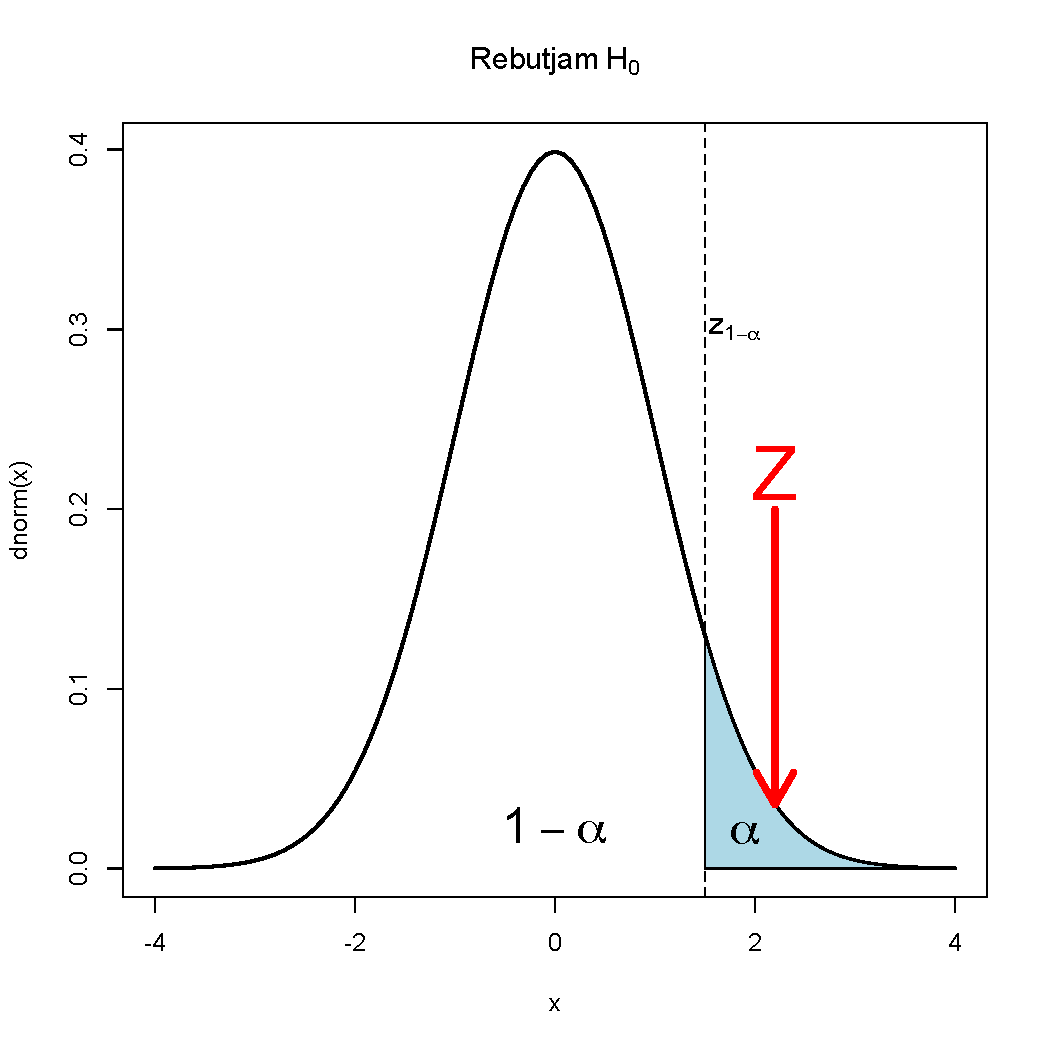
\includegraphics[width=0.7\linewidth]{rebutjamH0z.pdf}
\end{center}

\end{frame}


\begin{frame}
\frametitle{Ejemplo: C.H. para la media $\mu$ de normal con $\sigma$ conocida}
\vspace*{-0.75cm}

$$
\left\{\begin{array}{l}
H_{0}:\mu=\mu_{0}\\ H_{1}:\mu>\mu_{0}
\end{array}
\right.
$$
\begin{center}
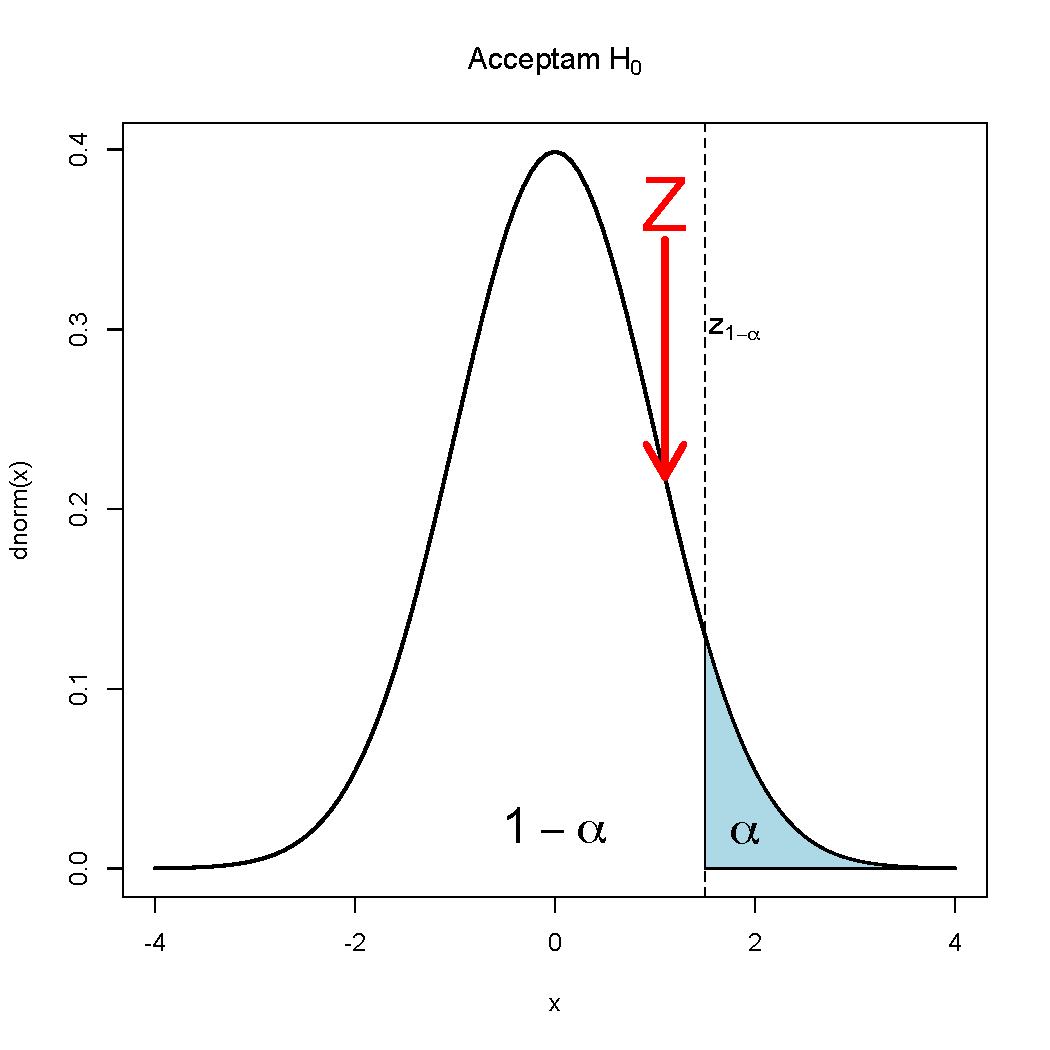
\includegraphics[width=0.7\linewidth]{acceptamH0z.pdf}
\end{center}

\end{frame}




\begin{frame}
\frametitle{Terminología}
Dado un contraste:
\medskip

\begin{itemize}
\item \emph{Estadístico de contraste}: el que
nos permite definir una regla de rechazo de $H_{0}$
\medskip

\item \emph{Nivel de significación $\alpha$}:  la probabilidad (máxima) de error de Tipo I
\medskip


\item \emph{Región crítica o de rechazo}:
si el estadístico de contraste pertenece a la región crítica, entonces rechazamos$H_{0}$
\medskip

\item \emph{Región de aceptación}:  el complementario de la región
crítica
\end{itemize}

\end{frame}

\begin{frame}
\frametitle{Terminología}
Dado un contraste:
\medskip

\begin{itemize}

\item \emph{Intervalo de confianza del $(1-\alpha)\cdot 100\%$}:  un intervalo  en el que el parámetro poblacional tiene probabilidad $1-\alpha$ de pertenecer (en el sentido de los intervalos de confianza del tema anterior)\\
\medskip

Se suele obtener imponiendo que el estadístico pertenezca a la región de aceptación para al nivel de significación   $\alpha$ y despejando el parámetro


\end{itemize}

\end{frame}

\begin{frame}
\frametitle{Ejemplo: C.H. para a $\mu$ de normal con $\sigma$ conocida}

Si la población es normal con $\sigma$ conocida,  un contraste    al nivel   de significación   $\alpha$ de
$$
\left\{\begin{array}{l}
H_{0}:\mu=\mu_{0}\\ H_{1}:\mu>\mu_{0}
\end{array}
\right.
$$
tiene 
\begin{itemize}
\item \emph{Estadístico de contraste}: $Z=
\dfrac{\overline{X}-\mu_{0}}{\frac{\sigma}{\sqrt{n}}}$
\medskip

\item \emph{Región crítica}: $]z_{1-\alpha},\infty[$
\medskip

\item \emph{Región de aceptación}: $]-\infty,z_{1-\alpha}]$
\medskip

\item \emph{Regla de decisión}:
rechazar   $H_{0}$ si
$Z>z_{1-\alpha}$
\end{itemize}
\end{frame}


\begin{frame}
\frametitle{Ejemplo: C.H. para a $\mu$ de normal con $\sigma$ conocida}

\begin{itemize}
\item \emph{Intervalo de confianza}: 
$$
\begin{array}{l}
\displaystyle Z\leq  z_{1-\alpha}\Longleftrightarrow  \dfrac{\overline{X}-\mu_{0}}{\frac{\sigma}{\sqrt{n}}}\leq  z_{1-\alpha} \\[2ex]
\displaystyle\qquad\quad\Longleftrightarrow  \mu_0\geq \overline{X}-z_{1-\alpha}\cdot\frac{\sigma}{\sqrt{n}}\\[2ex]
\displaystyle\qquad\quad\Longleftrightarrow \mu_0\in \red{\Big[\overline{X}-z_{1-\alpha}\cdot\frac{\sigma}{\sqrt{n}},\infty\Big[}
\end{array}
$$
Es
$$
\Big[\overline{X}-z_{1-\alpha}\cdot\frac{\sigma}{\sqrt{n}},\infty\Big[
$$
\medskip


\item \emph{Regla de decisión II}:
rechazar   $H_{0}$ si el $\mu_0$ contrastado no pertenece  al intervalo de confianza
\end{itemize}
\end{frame}


\begin{frame}
\frametitle{Ejemplo}
Sea $X$ una población normal con $\sigma=1.8$. Queremos hacer el contraste
$$
\left\{\begin{array}{l}
H_{0}:\mu=20\\ H_{1}:\mu>20
\end{array}
\right.
$$
con un nivel   de significación   de $0.05$
\medskip

Tomamos una m.a.s. de $n=25$ observaciones y obtenemos  $\overline{x}=20.25$
\medskip

¿Qué decidimos?
\end{frame}


\begin{frame}
\frametitle{Ejemplo}
$$
\left\{\begin{array}{l}
H_{0}:\mu=20\\ H_{1}:\mu>20
\end{array}
\right.
$$
$\alpha=0.05$, $\sigma=1.8$, $n=25$, $\overline{x}=20.25$
%\pause
\medskip

\begin{itemize}
\item \emph{Estadístico de contraste}: $Z=
\dfrac{\overline{X}-20}{\frac{1.8}{\sqrt{25}}}$
\medskip

\item Toma el valor $z_0=\dfrac{20.25-20}{\frac{1.8}{\sqrt{25}}}=0.694$
%\pause
\medskip

\item \emph{Región crítica}: $]z_{1-0.05},\infty[=]1.64,\infty[$
%\pause
\medskip

\item \emph{Decisión}: Como que $0.694<1.64$, no podemos rechazar   $H_0$
\end{itemize}

\end{frame}


\begin{frame}
\frametitle{Ejemplo}
$$
\left\{\begin{array}{l}
H_{0}:\mu=20\\ H_{1}:\mu>20
\end{array}
\right.
$$
$\alpha=0.05$, $\sigma=1.8$, $n=25$, $\overline{x}=20.25$
\medskip

\begin{itemize}

\item \emph{Intervalo de confianza}: 
$$
\Big[\overline{X}-z_{1-\alpha}\cdot\frac{\sigma}{\sqrt{n}},\infty\Big[=[19.66,\infty[
$$
%\pause
\medskip

\item \emph{Decisión}: Como que $20$ pertenece  al intervalo de confianza, no podemos rechazar   $H_0$
\end{itemize}

\end{frame}

\begin{frame}
\frametitle{Ejemplo}
Sea $X$ una población normal con $\sigma=1.8$. Queremos hacer el contraste
$$
\left\{\begin{array}{l}
H_{0}:\mu=20\\ H_{1}:\mu>20
\end{array}
\right.
$$
con un nivel   de significación   de $0.05$
\medskip

Tomamos una m.a.s. de $n=25$ observaciones y obtenemos  $\overline{x}=20.75$
\medskip

¿Qué decidimos?
\end{frame}


\begin{frame}
\frametitle{Ejemplo}
\vspace*{-4ex}

$$
\left\{\begin{array}{l}
H_{0}:\mu=20\\ H_{1}:\mu>20
\end{array}
\right.
$$
$\alpha=0.05$, $\sigma=1.8$, $n=25$, $\overline{x}=20.75$
%\pause
\medskip

\begin{itemize}
\item \emph{Estadístico de contraste}: $Z=
\dfrac{\overline{X}-20}{\frac{1.8}{\sqrt{25}}}$
\medskip

\item Toma el valor $z_0=\dfrac{20.75-20}{\frac{1.8}{\sqrt{25}}}=2.083$
%\pause\medskip

\item \emph{Región crítica}: $]z_{1-0.05},\infty[=]1.64,\infty[$
\medskip

\item \emph{Intervalo de confianza}: $[\overline{X}-z_{1-\alpha}\cdot\frac{\sigma}{\sqrt{n}},\infty[=[20.16,\infty[$
%\pause
\medskip

\item \emph{Decisión}: Rechazamos  $H_0$: Concluimos  que $\mu>20$
\end{itemize}

\end{frame}





\begin{frame}
\frametitle{Ejemplo}
Sea $X$ una población normal con $\sigma=1.8$. Queremos hacer el contraste
$$
\left\{\begin{array}{l}
H_{0}:\mu=20\\ H_{1}:\mu>20
\end{array}
\right.
$$
con un nivel   de significación   de $0.05$
\medskip

Tomamos una m.a.s. de $n=25$ observaciones y obtenemos  $\overline{x}=19.75$
\medskip

¿Qué decidimos?
%\pause
\medskip

Queremos rechazar $H_0$ contra $H_1$, si  $\overline{x}<20$? (\blue{Ejercicio:} Haced el cálculo, si no nos creéis)
\end{frame}




%%%%%%%

\begin{frame}
\frametitle{Ejemplo: C.H. para a $\mu$ de normal con $\sigma$ conocida}

Sea $X$ una v.a. $N(\mu,\sigma)$ con $\mu$ desconocida y $\sigma$ conocida
\medskip

Sea  $X_{1},\ldots,X_{n}$ una m.a.s. de $X$ de tamaño $n$
\medskip

Consideremos  el contraste
$$
\left\{\begin{array}{l}
H_{0}:\mu=\mu_{0}\\ H_{1}:\mu\ \red{<}\ \mu_{0}
\end{array}
\right.
$$
\medskip

rechazar   $H_{0}$ si $Z=\dfrac{\overline{X}-\mu_{0}}{{\sigma}/{\sqrt{n}}}$ es \emph{inferior a} un cierto umbral, que determinaremos con $\alpha$
\end{frame}

\begin{frame}
\frametitle{Ejemplo: C.H. para una media poblacional  $\mu$ de una distribución normal con $\sigma$ conocida}
\vspace*{-0.75cm}

$$
\left\{\begin{array}{l}
H_{0}:\mu=\mu_{0}\\ H_{1}:\mu\ \red{<}\ \mu_{0}
\end{array}
\right.
$$
Queremos
$$
\begin{array}{rl}
\alpha & =P(\mbox{rechazar   } H_{0}| H_{0} \mbox{ cierta})\\ 
& =P(Z<\mbox{umbral  })\Longrightarrow \red{\mbox{umbral  }=z_{\alpha}}
\end{array}
$$
por lo tanto,  para que  el nivel   de significación   del contraste    Sea $\alpha$,  la
\red{regla de rechazo} tiene que ser
$$
\red{Z<z_{\alpha}}
$$
La Región crítica es $]-\infty,z_{\alpha}[$
\end{frame}




\begin{frame}
\frametitle{Ejemplo: C.H. para la media   $\mu$ de una población   normal con $\sigma$ conocida}

Sea $X$ una v.a. $N(\mu,\sigma)$ con $\mu$ desconocida y $\sigma$ conocida
\medskip

Sea  $X_{1},\ldots,X_{n}$ una m.a.s. de $X$ de tamaño $n$
\medskip

Consideremos  el contraste
$$
\left\{\begin{array}{l}
H_{0}:\mu=\mu_{0}\\ H_{1}:\mu\ \red{\neq}\ \mu_{0}
\end{array}
\right.
$$
\medskip

Rechazar $H_{0}$ si $Z=\dfrac{\overline{X}-\mu_{0}}{{\sigma}/{\sqrt{n}}}$ está a \emph{bastante lejos de} de 0, y la determinaremos con el valor de  $\alpha$
\end{frame}

\begin{frame}
\frametitle{Ejemplo: C.H. para la media   $\mu$ de una población   normal con $\sigma$ conocida}


$$
\left\{\begin{array}{l}
H_{0}:\mu=\mu_{0}\\ H_{1}:\mu\ \red{\neq}\ \mu_{0}
\end{array}
\right.
$$
Queremos
$$
\begin{array}{rl}
\alpha & =P(\mbox{rechazar   } H_{0}| H_{0} \mbox{ cierta })\\ 
& =P(Z<-\mbox{umbral  }\mbox{ o }Z>\mbox{umbral  })\\
& =P(Z<-\mbox{umbral  })\!+\!P(Z>\mbox{umbral  })\\
& = 2P(Z>\mbox{umbral  })=2(1-P(Z<\mbox{umbral  }))\\
& \qquad \Longrightarrow P(Z<\mbox{umbral  })=1-\dfrac{\alpha}{2}\\
&  \qquad \Longrightarrow \red{\mbox{umbral  }=z_{1-\frac{\alpha}{2}}}
\end{array}
$$
\end{frame}

\begin{frame}
\frametitle{Ejemplo: C.H. para la media   $\mu$ de una población   normal con $\sigma$ conocida}


$$
\left\{\begin{array}{l}
H_{0}:\mu=\mu_{0}\\ H_{1}:\mu\ \red{\neq}\ \mu_{0}
\end{array}
\right.
$$
\medskip

ahora para que el nivel de significación del contraste sea $\alpha$,  la
regla de rechazo tiene que ser
$$
\red{Z<-z_{1-\frac{\alpha}2}=z_{\frac{\alpha}2}\mbox{ o }Z>z_{1-\frac{\alpha}2}}
$$
La región crítica es $]-\infty,z_{\frac\alpha2}[\cup ]z_{1-\frac{\alpha}2},\infty[$
\end{frame}


\begin{frame}
\frametitle{Ejemplo: C.H. para la media   $\mu$ de una población   normal con $\sigma$ conocida}

\vspace*{-0.75cm}

$$
\left\{\begin{array}{l}
H_{0}:\mu=\mu_{0}\\ H_{1}:\mu\neq\mu_{0}
\end{array}
\right.
$$
\begin{center}
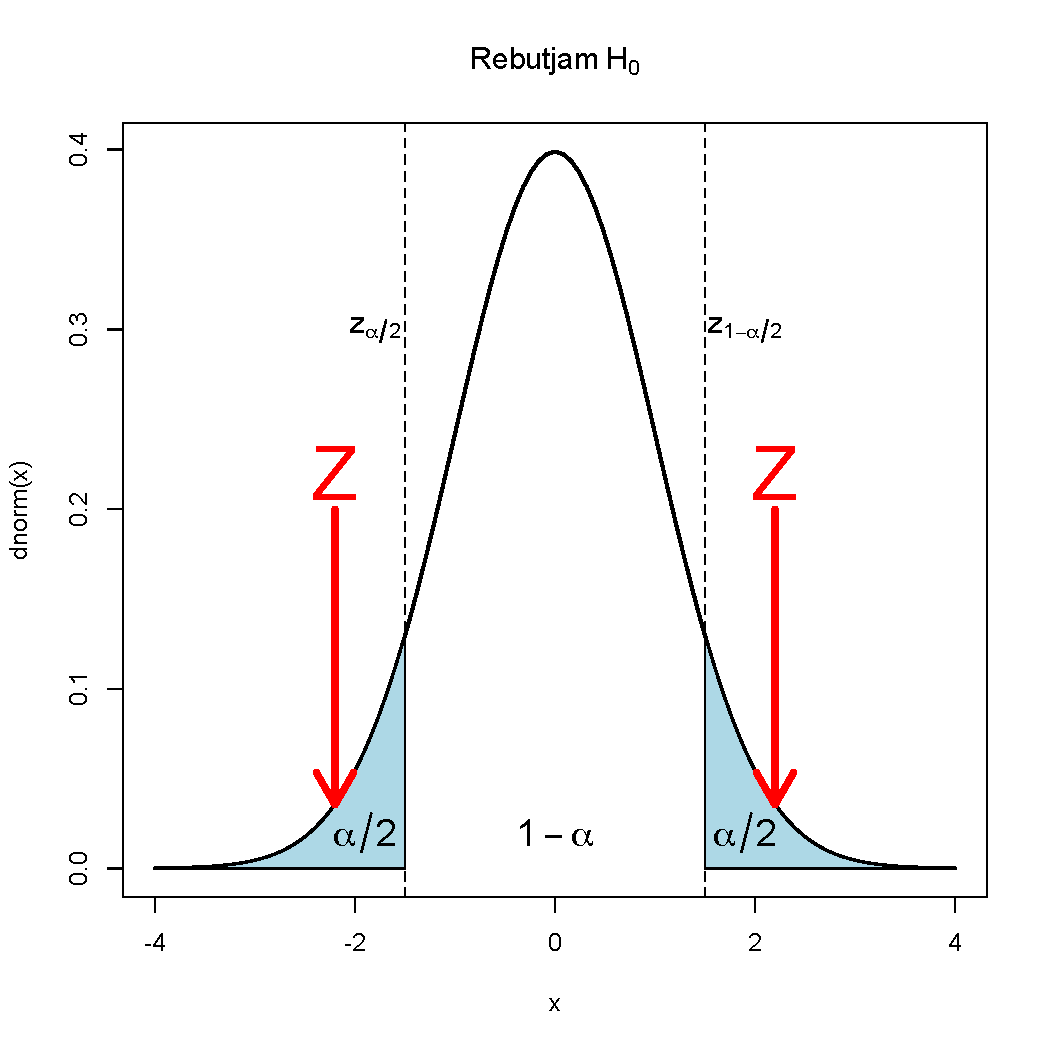
\includegraphics[width=0.7\linewidth]{rebutjamH0z2.pdf}
\end{center}

\end{frame}

\begin{frame}
\frametitle{Ejemplo: C.H. para la media   $\mu$ de una población   normal con $\sigma$ conocida}

\vspace*{-0.75cm}

$$
\left\{\begin{array}{l}
H_{0}:\mu=\mu_{0}\\ H_{1}:\mu\neq\mu_{0}
\end{array}
\right.
$$
\begin{center}
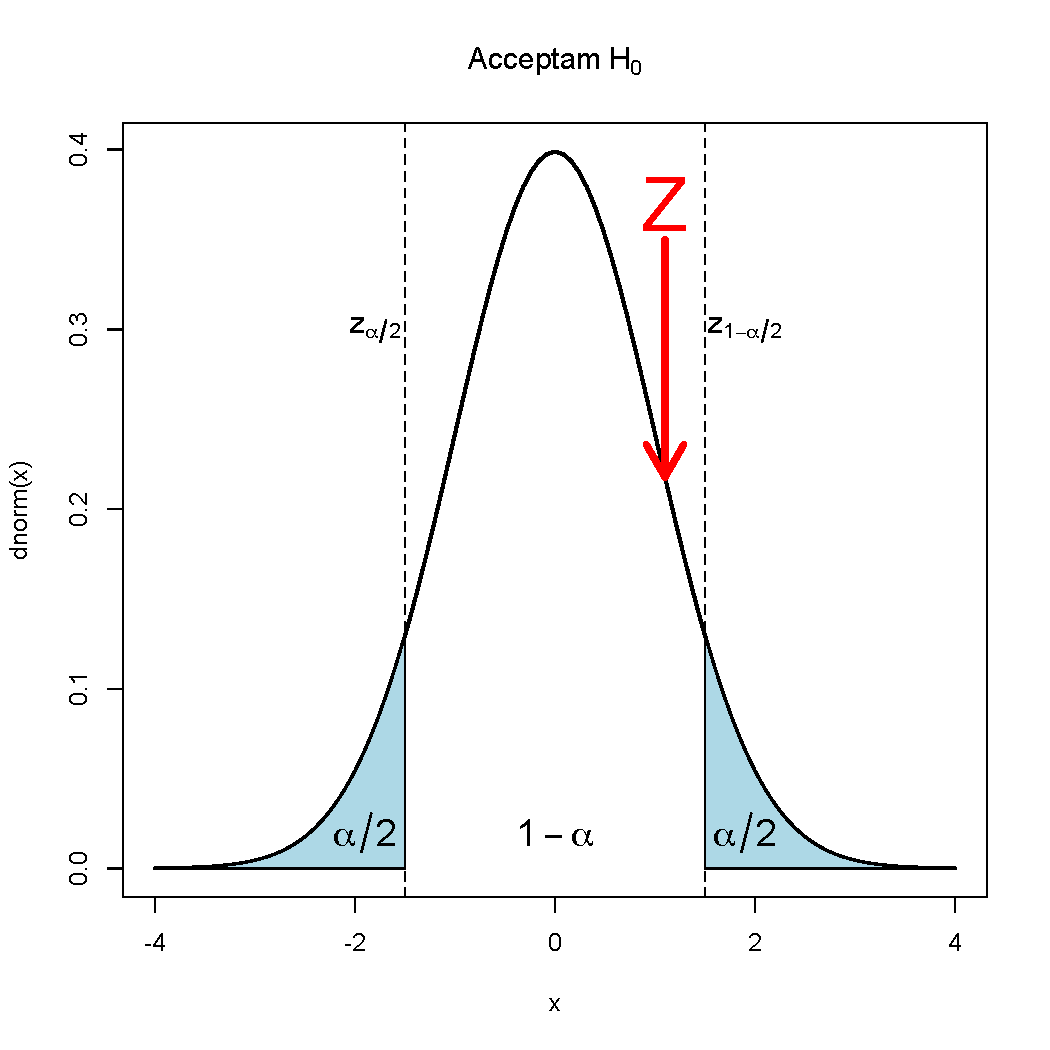
\includegraphics[width=0.7\linewidth]{acceptamH0z2.pdf}
\end{center}

\end{frame}





\begin{frame}
\frametitle{Ejemplo: C.H. para la media   $\mu$ de una población   normal con $\sigma$ conocida}

\vspace*{-0.75cm}

$$
\left\{\begin{array}{l}
H_{0}:\mu=\mu_{0}\\ H_{1}:\mu\ \red{\neq}\ \mu_{0}
\end{array}
\right.
$$
¿Intervalo de confianza?
$$
\begin{array}{l}
\displaystyle -z_{1-\frac{\alpha}2}\leq Z\leq z_{1-\frac{\alpha}2}\Longleftrightarrow -z_{1-\frac{\alpha}2}\leq \dfrac{\overline{X}-\mu_0}{\frac{\sigma}{\sqrt{n}}}\leq z_{1-\frac{\alpha}2}\\[2ex]
 \displaystyle\qquad\Longleftrightarrow -z_{1-\frac{\alpha}2}\frac{\sigma}{\sqrt{n}}\leq \overline{X}-\mu_0\leq z_{1-\frac{\alpha}2}\frac{\sigma}{\sqrt{n}} \\[2ex]
\displaystyle  \qquad\Longleftrightarrow \overline{X}-z_{1-\frac\alpha2}\frac{\sigma}{\sqrt{n}}\leq \mu_0\leq \overline{X}+z_{1-\frac{\alpha}2}\frac{\sigma}{\sqrt{n}} \\[2ex]
\displaystyle  \qquad\Longleftrightarrow\mu_0\in \red{\Big[\overline{X}-z_{1-\frac\alpha2}\frac{\sigma}{\sqrt{n}},\overline{X}+z_{1-\frac{\alpha}2}\frac{\sigma}{\sqrt{n}}\Big]}
   \end{array}
$$
¿Os recuerda a algo\ldots?
\end{frame}





\begin{frame}
\frametitle{Ejemplo}
Sea $X$ una población normal con $\sigma=1.8$. Queremos realizar el contraste
$$
\left\{\begin{array}{l}
H_{0}:\mu=20\\ H_{1}:\mu\neq 20
\end{array}
\right.
$$
con un nivel   de significación   de $0.05$
\medskip

Tomamos una m.a.s. de $n=25$ observaciones y obtenemos  $\overline{x}=20.5$
\medskip

¿Qué decidimos?
\end{frame}


\begin{frame}
\frametitle{Ejemplo}
\vspace*{-4ex}

$$
\left\{\begin{array}{l}
H_{0}:\mu=20\\ H_{1}:\mu\neq 20
\end{array}
\right.
$$
$\alpha=0.05$, $\sigma=1.8$, $n=25$, $\overline{x}=20.5$
%\pause
\medskip

\begin{itemize}
\item \emph{Estadístico de contraste}: $Z=
\dfrac{\overline{X}-20}{\frac{1.8}{\sqrt{25}}}$
\medskip

\item Toma el valor $z_0=\dfrac{20.5-20}{\frac{1.8}{\sqrt{25}}}=1.39$
%\pause
\medskip

\item \emph{Región crítica}: $]-\infty,z_{0.025}[\cup ]z_{0.975},\infty[$=$]-\infty,-1.96[\cup ]1.96,\infty[$
\medskip

\item \emph{Intervalo de confianza}: $[19.794,21.206]$
%\pause
\medskip

\item \emph{Decisión}:
No podemos  rechazar   $H_0$
\end{itemize}

\end{frame}




\subsection{$p$-valor}

\begin{frame}
\frametitle{El $p$-valor}

El  \emph{$p$-valor} o  \emph{valor crítico}  ($p$-\textsl{value}) de un contraste es la probabilidad que, si $H_0$ es verdadera, el estadístico de contraste tome un valor tan extremo o  más que el que se ha observado
\medskip

\blue{Ejemplo:} En un contraste
$$
\left\{\begin{array}{l}
H_{0}:\mu=\mu_{0}\\ H_{1}:\mu\ \red{>}\ \mu_{0}
\end{array}
\right.
$$
si el estadístico $Z$ tiene el  valor $z_0$,
$$
\mbox{$p$-valor}=P(Z\ \red{\geq}\ z_0)
$$ 
\end{frame}



\begin{frame}
\frametitle{El $p$-valor}
\vspace*{-0.75cm}

$$
\left\{\begin{array}{l}
H_{0}:\mu=\mu_{0}\\ H_{1}:\mu>\mu_{0}
\end{array}
\right.
$$
\begin{center}
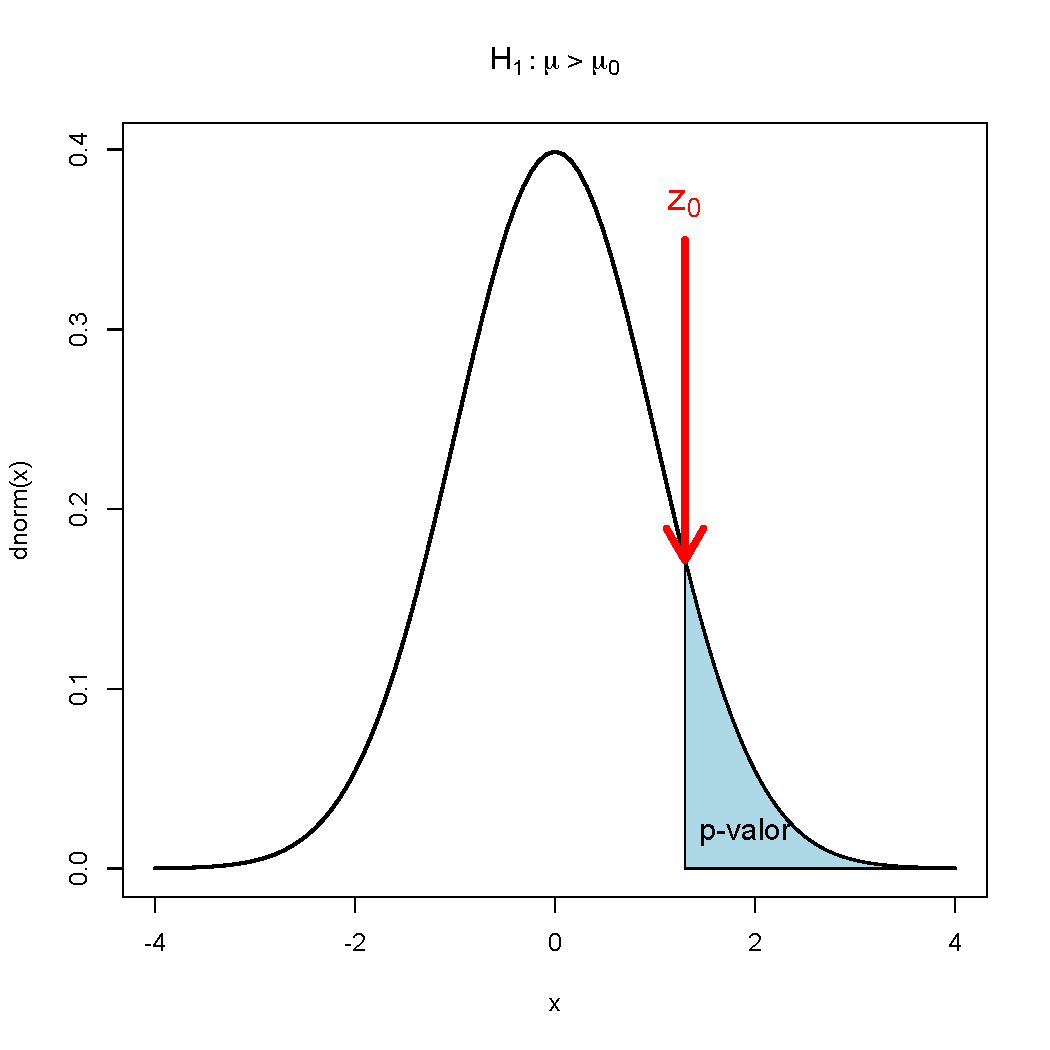
\includegraphics[width=0.7\linewidth]{pvalor01.pdf}
\end{center}

\end{frame}



\begin{frame}
\frametitle{El $p$-valor}

El  \emph{$p$-valor} o  \emph{valor crítico}  ($p$-\textsl{value}) de un contraste es la probabilidad que, si $H_0$ es verdadera, el estadístico de contraste tome un valor tan extremo o  más que el que se ha observado
\medskip

\blue{Ejemplo:} En un contraste
$$
\left\{\begin{array}{l}
H_{0}:\mu=\mu_{0}\\ H_{1}:\mu\ \red{<}\ \mu_{0}
\end{array}
\right.
$$
si el estadístico $Z$  es  $z_0$,
$$
\mbox{$p$-valor}=P(Z\ \red{\leq}\ z_0)
$$
\end{frame}

\begin{frame}
\frametitle{El $p$-valor}
\vspace*{-0.75cm}

$$
\left\{\begin{array}{l}
H_{0}:\mu=\mu_{0}\\ H_{1}:\mu<\mu_{0}
\end{array}
\right.
$$
\begin{center}
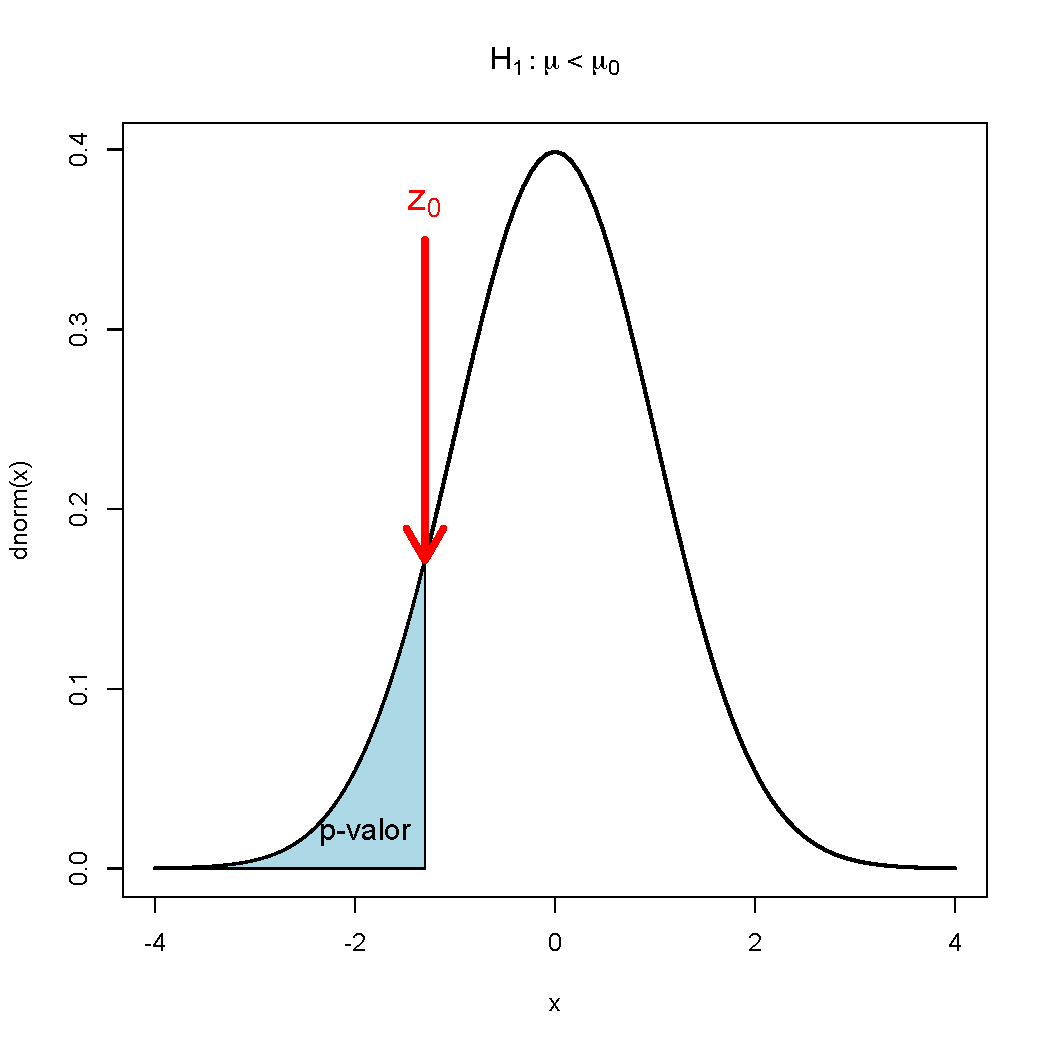
\includegraphics[width=0.7\linewidth]{pvalor10.pdf}
\end{center}

\end{frame}


\begin{frame}
\frametitle{El $p$-valor}

El  \emph{$p$-valor} o  \emph{valor crítico}  ($p$-\textsl{value}) de un contraste es la probabilidad que, si $H_0$ es verdadera, el estadístico de contraste tome un valor tan extremo o  más que el que se ha observado
\medskip

\blue{Ejemplo:} En un contraste
$$
\left\{\begin{array}{l}
H_{0}:\mu=\mu_{0}\\ H_{1}:\mu\ \red{\neq}\ \mu_{0}
\end{array}
\right.
$$
si el estadístico $Z$ ha dado  $z_0$,
$$
\begin{array}{rl}
\mbox{$p$-valor} & =2\cdot \min\{P(Z\ \red{\leq} -|z_0|),P(Z\ \red{\geq}\ |z_0|)\}\\
 & =2\cdot P(Z\ \red{\geq}\ |z_0|)
\end{array}
$$
\end{frame}



\begin{frame}
\frametitle{El $p$-valor}
\vspace*{-0.75cm}

$$
\left\{\begin{array}{l}
H_{0}:\mu=\mu_{0}\\ H_{1}:\mu\neq\mu_{0}
\end{array}
\right.
$$
\begin{center}
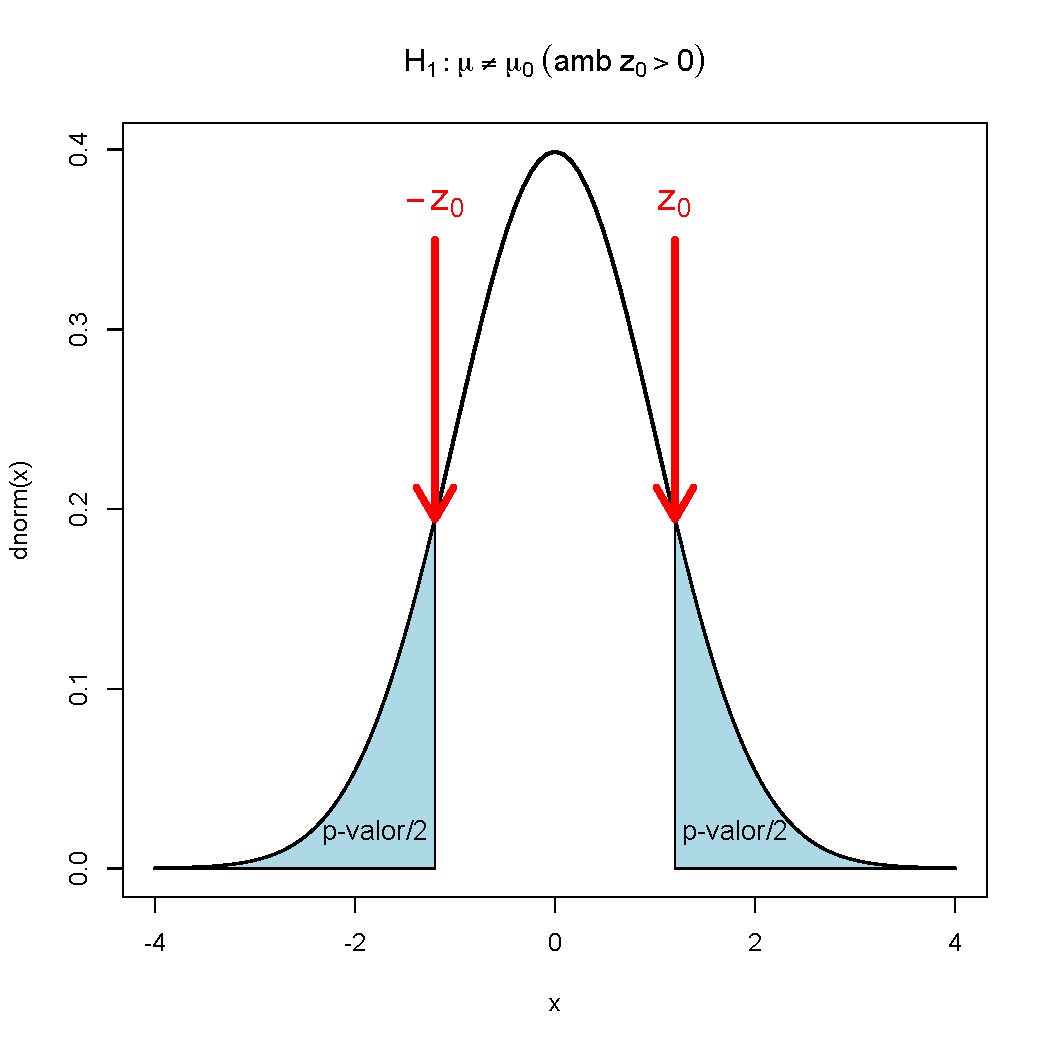
\includegraphics[width=0.7\linewidth]{pvalor11.pdf}
\end{center}

\end{frame}


\begin{frame}
\frametitle{El $p$-valor}

El  \emph{$p$-valor} o  \emph{valor crítico}  ($p$-\textsl{value}) de un contraste es la probabilidad que, si $H_0$ es verdadera, el estadístico de contraste tome un valor tan extremo o  más que el que se ha observado
\bigskip


Es una  \emph{medida inversa de la fuerza de las pruebas o evidencias que hay en contra de $H_1$}: si $H_0$ es verdadera, cuanto más pequeño sea el $p$-valor, más improbable es observar lo  que hemos observado. 
\medskip

en consecuencia, cuanto  más pequeño sea el $p$-valor, con más fuerza podemos rechazar $H_0$.
\end{frame}




\begin{frame}
\frametitle{El $p$-valor}

\blue{por ejemplo tomemos,} $p$-valor${} =0.03$ 
\medskip

\begin{itemize}
\item \emph{Significa} que la probabilidad que, si $H_0$ es verdadera, el estadístico de contraste tome un valor tan extremo o más que el que ha pres  es 0.03 (pequeño: evidencia que $H_0$ es falsa)
\medskip

\item \emph{No significa}:
\medskip

\begin{itemize}
\item La probabilidad que $H_0$ Sea verdadera   es $0.03$
\medskip

\item  $H_0$ es verdadera   un 3\% de les veces
\end{itemize}
\end{itemize}
\end{frame}






\begin{frame}
\frametitle{El $p$-valor}
\vspace*{-3ex}

\begin{block}{¡Importante!}
En un contraste con nivel de significación   $\alpha$, 
\begin{itemize}
\item rechazamos $H_0$ si $p$-valor $<\alpha$

\item aceptamos $H_0$ si $\alpha\leq p$-valor
\end{itemize}
\end{block}
\medskip

\blue{Ejemplo:} En un contraste
$$
\left\{\begin{array}{l}
H_{0}:\mu=\mu_{0}\\ H_{1}:\mu> \mu_{0}
\end{array}
\right.
$$

supongamos  que el estadístico $Z$ vale $z_0$. El $p$-valor es $P(Z \geq z_0)$
$$
\begin{array}{l}
\hspace*{-2ex}\mbox{Rechazamos }  H_0  \Longleftrightarrow z_0>z_{1-\alpha}\\
 \Longleftrightarrow P(Z \geq z_0)<P(Z\geq z_{1-\alpha})=1-(1-\alpha)=\alpha
\end{array}
$$
\end{frame}

\begin{frame}
\frametitle{El $p$-valor}
\vspace*{-3ex}

\begin{block}{¡Importante!}
En un contraste con nivel   de significación   $\alpha$, 
\begin{itemize}
\item rechazamos $H_0$ si $p$-valor $<\alpha$

\item aceptamos $H_0$ si $\alpha\leq p$-valor
\end{itemize}
\end{block}
\medskip

\blue{Ejemplo:} En un contraste
$$
\left\{\begin{array}{l}
H_{0}:\mu=\mu_{0}\\ H_{1}:\mu \neq \mu_{0}
\end{array}
\right.
$$
supongamos  que el estadístico $Z$ vale $z_0>0$. El $p$-valor es $2P(Z \geq z_0)$
$$
\begin{array}{l}
\hspace*{-2ex}\mbox{Rechazamos }  H_0  \Longleftrightarrow z_0>z_{1-\frac{\alpha}{2}}\\
 \Longleftrightarrow 2P(Z \geq z_0)<2P(Z\geq z_{1-\frac{\alpha}{2}})=2(1-(1-\frac{\alpha}{2}))=\alpha
\end{array}
$$
\end{frame}



\begin{frame}
\frametitle{El $p$-valor}
\vspace*{-3ex}

\begin{block}{Importante!}
En un contraste con nivel de significación $\alpha$, 
\begin{itemize}
\item rechazamos $H_0$ si $p$-valor $<\alpha$

\item aceptamos $H_0$ si $\alpha\leq p$-valor
\end{itemize}
\end{block}
\medskip

El  \emph{$p$-valor}  de un contraste    es 
\begin{itemize}
\item  El nivel   de significación   $\alpha$ más pequeño para el que rechazamos  la hipótesis nula
\medskip

\item El nivel   de significación   $\alpha$ más grande para el que aceptaríamos la hipótesis nula
\medskip

%\only<2>{
\item \blue{La probabilidad mínima de error de Tipo  I que permitimos  si rechazamos la hipótesis nula con el valor del estadístico de contraste obtenido}
%}

%\only<3>{
\item \blue{La probabilidad máxima de error de Tipo  I que permitimos  si aceptamos la hipótesis nula con el valor del estadístico de contraste
obtenido}
%}
\end{itemize}
\end{frame}



\begin{frame}[fragile]
\frametitle{El $p$-valor}
\vspace*{-3ex}

\begin{block}{¡Importante!}
Si no establecemos un nivel   de significación   $\alpha$, entonces
\begin{itemize}
\item Aceptamos $H_0$ si el $p$-valor es ``grande'' ($\geq 0.1$)
\medskip

\item Rechazamos $H_0$ si el $p$-valor es ``pequeño'' ($<0.05$). En este caso, el $p$-valor es 
\begin{itemize}
\item \emph{Significativo} si es $< 0.05$
\item \emph{Fuertemente significativo} si es $<0.01$
\item \emph{Muy significativo} si es $<0.001$
\end{itemize}
\end{itemize}
\end{block}
{\small \begin{verbatim}
Signif. codes: 0‘***’0.001‘**’0.01‘*’0.05‘.’0.1‘ ’1 
\end{verbatim}
}\medskip

Si el $p$-valor está entre $0.05$ y $0.1$ y no tenemos nivel de significación, se requieren¡ estudios posteriores para tomar una decisión ("la \emph{zona crepuscular}, \textsl{twilight zone}")

\end{frame}


\begin{frame}
\frametitle{Ejemplo}
Sea $X$ una población normal con $\sigma=1.8$. Queremos hacer el contraste
$$
\left\{\begin{array}{l}
H_{0}:\mu=20\\ H_{1}:\mu>20
\end{array}
\right.
$$
\medskip

Tomamos una m.a.s. de $n=25$ observaciones y obtenemos  $\overline{x}=20.25$
\medskip

¿Qué decidimos?%\pause

\medskip No tenemos $\alpha$: Observamos  el $p$-valor
\end{frame}


\begin{frame}
\frametitle{Ejemplo}

\begin{itemize}
\item \emph{Estadístico de contraste}: $Z=
\dfrac{\overline{X}-20}{\frac{1.8}{\sqrt{25}}}$
\medskip

Toma el valor $z_0=\dfrac{20.25-20}{\frac{1.8}{\sqrt{25}}}=0.694$
%\pause\medskip

\item \red{$p$-valor}$=P(Z\geq 0.694)=0.2438>0.1$ gran
%\pause\medskip

\item \emph{Decisión}:
No podemos rechazar   $H_{0}$
\end{itemize}

\end{frame}


\begin{frame}
\frametitle{Ejemplo}
Sea $X$ una población normal con $\sigma=1.8$. Queremos hacer el contraste
$$
\left\{\begin{array}{l}
H_{0}:\mu=20\\ H_{1}:\mu>20
\end{array}
\right.
$$
\medskip

Tomamos una m.a.s. de $n=25$ observaciones y obtenemos  \red{$\overline{x}=20.75$}
\medskip

¿Qué decidimos?

\end{frame}


\begin{frame}
\frametitle{Ejemplo}

\begin{itemize}
\item \emph{Estadístico de contraste}: $Z=
\dfrac{\overline{X}-20}{\frac{1.8}{\sqrt{25}}}$
\medskip

Toma el valor $z_0=\dfrac{20.75-20}{\frac{1.8}{\sqrt{25}}}=2.083$
%\pause\medskip

\item \red{$p$-valor}$=P(Z\geq 2.083)=0.0186$  pequeño
%\pause\medskip

\item \emph{Decisión}:
Rechazamos $H_{0}$ contra $H_1$
\end{itemize}

\end{frame}


\begin{frame}
\frametitle{Decisiones}

Podemos decidir un contraste:
\begin{itemize}
\item \emph{con la regio crítica:} Si el estadístico de contraste    cae dentro la Región crítica para al nivel   de significación   $\alpha$, rechazamos$H_0$
\medskip

\item \emph{con el intervalo de confianza:} Si el parámetro poblacional a contrastar cae dentro el intervalo de confianza para al nivel   $(1-\alpha)\cdot 100\%$, aceptamos $H_0$
\medskip

\item \emph{con el $p$-valor:} Si el $p$-valor es más pequeño que el nivel   de significación   $\alpha$, rechazamos $H_0$
\medskip

\item \emph{con el $p$-valor y sin $\alpha$:} Si el $p$-valor es pequeño, rechazamos $H_0$, y si es grande,  aceptamos
\end{itemize}
\medskip

\blue{Aquí utilizaremos el $p$-valor}
\end{frame}



\subsection{Los pasos de un contraste}

\begin{frame}
\frametitle{El método de los \emph{seis} pasos (con $\alpha$)}

\begin{enumerate}[1)]
\item Establecer   la hipótesis nula  $H_{0}$   y la hipótesis alternativa  $H_{1}$
\smallskip

\item  Fijar un nivel   de significación   $\alpha$
\smallskip

\item Seleccionar el estadístico de contraste    apropiado 
\smallskip

\item Calcular el valor del estadístico de contraste a partir de les
datos muestrales
\smallskip

\item  Calcular el $p$-valor del contraste
\smallskip

\item \emph{Decisión:} rechazar $H_{0}$ en favor de $H_1$  si el $p$-valor es 
más pequeño que $\alpha$; en caso contrario, aceptar $H_{0}$
\end{enumerate}
\end{frame}


\begin{frame}
\frametitle{El método de los \emph{cinco} pasos (sin $\alpha$)}

\begin{enumerate}[1)]
\item Establecer   la hipótesis nula  $H_{0}$   y la hipótesis alternativa  $H_{1}$
\smallskip

\item Seleccionar el estadístico de contraste apropiado
\smallskip

\item Calcular el valor del estadístico de contraste a partir de los valores de la muestra
\smallskip

\item  Calcular el $p$-valor del contraste
\smallskip

\item \emph{Decisión:} rechazar $H_{0}$ en favor de $H_1$  si el $p$-valor es pequeño ($<0.05$), aceptar $H_{0}$ si el $p$-valor es grande ($\geq 0.1$), y ampliar el estudio si el $p$-valor está entre 0.05 y 0.1
\end{enumerate}
\end{frame}






\begin{frame}
\frametitle{Ejemplo}

Los años de vida de un  router sigue  aproximadamente una ley de distribución normal con $\sigma=0.89$ años
\medskip

Una muestra aleatoria de la duración de 100 aparatos ha dado una vida media de 7.18 años
\medskip

Queremos decidir si la vida media en de estos routers es superior a  7 años
\medskip

utilizaremos el contraste
$$
\left\{\begin{array}{l}
H_{0}:\mu=7\\ 
H_{1}:\mu>7
\end{array}
\right.
$$
\end{frame}

\begin{frame}
\frametitle{Ejemplo: con $\alpha$}

Tomamos  un nivel   de significación   $\alpha=0.05$
\medskip

EL estadístico  de contraste    es 
$$
Z=\frac{\overline{X}-7}{0.89/\sqrt{100}}=\frac{\overline{X}-7}{0.089}
$$
El valor en este contraste  es $z_0\!=\!\dfrac{71.8-70}{0.89}\!=\!2.02$
\medskip

El $p$-valor es 
$$
P(Z\geq 2.02)=0.0217
$$
Como  $0.0217<\alpha$, rechazamos $H_0$: concluimos que $\mu>70$

\end{frame}


\begin{frame}
\frametitle{Ejemplo: con $\alpha$}

\red{Supongamos  que tomamos  un nivel  de significación   $\alpha=0.01$}
\medskip

El estadístico  de contraste    es 
$$
Z=\frac{\overline{X}-70}{6.8/\sqrt{100}}=\frac{\overline{X}-70}{0.68}
$$

El valor del estadístico de contraste con esta muestra es $z_0\!=\!\dfrac{71.8-70}{0.68}\!=\!2.022$
\medskip

El $p$-valor es 
$$
P(Z\geq 2.022)=0.0217
$$
\red{Como $0.0217>\alpha$, no podemos rechazar   $H_0$: concluimos que $\mu\leq 70$ con este nivel de significación}

\end{frame}




\begin{frame}
\frametitle{Ejemplo: sin $\alpha$}

El estadístico  de contraste    es 
$$
Z=\frac{\overline{X}-70}{6.8/\sqrt{100}}=\frac{\overline{X}-70}{0.68}
$$
Su valor en este contraste es $z_0\!=\!\dfrac{71.8-70}{0.68}\!=\!2.022$

\medskip

El $p$-valor es 
$$
P(Z> 2.022)=0.0216
$$
Como es pequeño ($<0.05$), rechazamos $H_0$: concluimos que $\mu>70$

\end{frame}

\begin{frame}
\frametitle{Un último consejo }

Como una regla recomendaríamos en un informe:
\medskip

\begin{itemize}
\item \emph{Si tenemos fijado (conocemos)  $\alpha$:} Encontrar el $p$-valor y el intervalo de confianza del contraste para $\alpha$ dado    (nivel   de confianza $(1-\alpha)\cdot 100\%$)
\medskip

\item \emph{Si no tenemos fijado (no conocemos) $\alpha$:} Encontrar el $p$-valor, y el intervalo de confianza del contraste al nivel  de confianza  $95\%$

\end{itemize}


\end{frame}




\end{document}
